\documentclass[twocolumn,9pt]{article}

\usepackage{mdframed}

% Handle enumeration list
\usepackage{enumitem}

\usepackage{amsmath}
\usepackage{amssymb}
\usepackage{graphicx}
\usepackage{microtype}

% Directory for images
\graphicspath{{images/}}

% To wrap text around figures
%\usepackage{wrapfig}
%\usepackage{caption}

% Define new type of columns
%\usepackage{array}
%\usepackage{tabulary}
%\newcolumntype{K}[1]{>{\centering\arraybackslash}m{#1}}

% Stretch the dimension of the rows in tables
%\renewcommand{\arraystretch}{1.6}

% Add colors to table
%\usepackage{colortbl}

% Set Helvetica as main font
\usepackage{helvet}
\renewcommand\familydefault{\sfdefault}
\usepackage[T1]{fontenc}

% Set Helvetica as main font for equations
\usepackage[helvet]{sfmath}

% Change geometry of the page
\usepackage[margin=0.8in]{geometry}

\usepackage[svgnames]{xcolor}
\usepackage[hidelinks]{hyperref}

% Redefine names
\newcommand{\sectionname}{Section}
\renewcommand{\appendixname}{Appendix}
\newcommand{\equationname}{Equation}
\newcommand{\referencename}{Ref.}
\renewcommand{\figurename}{Figure}
\renewcommand{\tablename}{Table}

% Some useful definition
\newcommand{\DW}{D-Wave 2X}


\begin{document}

\title{Notes on Quantum Annealing for Air Traffic Management}
\author{QuAIL Team}
\maketitle

\section*{Introduction}\label{sec:intro}
Building on our promising prior results in the planning domain~\cite{rieffel:15,venturelli:15},
we have begun to explore the potential of quantum annealing (QA) for solving challenging computational 
problems related to air traffic management (ATM)\cite{rodionova:16, rodionova:thesis15}.
This work is being performed by members of the QuAIL team (Tobias Stollenwerk, Bryan O'Gorman, 
Salvatore Mandr\`a, Davide Venturelli and Eleanor G. Rieffel) with expertise in all aspects of 
applying quantum annealing to real-world problems, in close collaboration with domain experts 
in ATM (Olga Rodionova, Hok K. Ng and Banavar Sridhar).
We have identified a specific problem within ATM to serve as a case study, and have made significant 
progress towards formulating it in a way that is amenable to quantum computing. As a concrete example 
of application for ATM, we focus on flight data in the North Atlantic oceanic airspace (NAT), 
for which we have wind-optimal trajectories for two consecutive days 
(July 28\textsuperscript{th}-29\textsuperscript{th} 2012) for which state-of-the-art solutions exist. 
The NAT dataset consists of wind-optimal trajectories in (3+1)-dimensions for 984 flights. 
These trajectories, subsets thereof, and toy-instances based thereon will serve as our benchmark set.

\section*{Formulation of the problem}\label{sec:approach}

The main challenge of applying quantum annealing to a real-world problem is in formulating
the problem as Quadratic Unconstrained Binary Optimization (QUBO), i.e.\ a quadratic real-valued
polynomial over Boolean-valued variables of the form
$$
    H = \sum_{(i,\,j)\in E} x_i Q_{ij} x_j,
$$
where $x_j$ are boolean variables, $Q_{ij}$ is a real-symmetric matrix and the only allowed couplings
are the edges of a given set $E$. The set of edges $E$ depends on the architecture of the quantum hardware.
%
In the specific case of the NAT dataset, we are focusing on the problem to minimize the total delay 
of a set of flights (each consisting of an origin, destination, and departure time).
More precisely, we are given the wind-optimal trajectories for every flight, 
and wish to choose a set of modifications of these trajectories so that they a) do not conflict
with each other, and b) minimize the sum of the delays of the flights at their destinations,
relative to the wind-optimal trajectories.
%
To do so, we first parameterize the trajectory modifications in such a way that a) the parameterizations
could be encoded in Boolean-valued variables, and b) the constraints and cost function
(total delay) could be expressed as quadratic polynomial over those bits.
The modifications to the trajectories that we consider are of two types:
\begin{itemize}
    \item The origination delays, in which the departure of the flight from its origin is
          simply delayed, and its trajectory translated in time only. 
    \item The avoidance maneuvers, in which flights may briefly change course in order to avoid
          conflicts with others; we assume that a maneuver is local so that the net effect is an
          effective delay at the conflict point.
\end{itemize}
%
Given the set of wind-optimal trajectories, we refer to the points in space that more than one trajectory 
crosses at some time ``spatial conflicts''. Since the state-of-art quantum hardware has a limited amount of
physical resources, we cannot take trace of all the possible spatial conflicts. 
To overcome this limitation, we introduce the concept of ``potential conflict'', namely the set
of all those conflict that ``potentially'' can happen within a certain time window $\theta$,
i.e. $|t_{i,k} - t_{j,k}| \leq \theta$ for two flights $i$ and $j$ at potential conflict $k$,
with $t_{i,k}$ be the variable indicating the time at which flight $i$ gets to potential conflict $k$.
Potential conflicts are then iteratively computed using a software developed internally at the QuAIL lab.

The next step consists in devise a binary model to resolve the potential conflicts. Let 
$t_{i,k}^*$ be the wind-optimal value at a certain potential conflict $k$. 
The difference between them $D_{i,k} = t_{i,k} - t^*_{i,k}$ 
is the accumulation of delays that flight $i$ encounters before conflict $i$.
Let $d_{i,k}$ be the variable indicating the delay added to flight $i$ at potential conflict $k$.
Then the delay can be written $D_{i,k} = d_i + \sum_{k' \in P_{i,k}} d_{i,k}$, 
where $d_i$ is the origination delay and $P_{i,k}$ is the set of potential conflicts that flight $i$ 
encounters prior to $k$.
This type of penalties can be done by encoding each time $t_{i,k} = \sum_{\alpha} \alpha t_{i,k,\alpha}$ 
using bits indicating its value from a discrete set $\{\alpha\}$, and adding the penalty term 
$\sum_{|\alpha - \beta| < \theta} t_{i,k,\alpha} t_{j,k,\beta}$.
We are currently exploring the relative advantages of encoding the trajectories using the absolute 
times $\{t_{i,k}\}$ or the relative delays $\{d_{i,k}\}$ (both lead to qualitatively similar resource 
requirements), as well as different ways of encoding the potential maneuvers, especially when multiple 
flights potentially conflict at the same point in space and time.

\section*{Analysis of the potential conflicts}

The first analysis we perform is related to the topology of the potential conflicts. The idea is to represent
the NAT dataset as a graph $\mathcal{G}$: each node of the graph is a flight and two flights are connected only if they
are involved in a potential conflicts. Connected components of the resulting graph represent the subset
of flights that share a potential conflict. Indeed, if two flights are in different connected components,
they never have a potential conflicts. Therefore, this implies that each connected component can be 
\emph{independently} solved. The graph $\mathcal{G}$ depends on the choice of the time window $\theta$
we use to compute the potential conflicts. However, we have observed that little changes by varying $\theta$ showing
that our definition of potential conflicts is robust. \figurename~\ref{fig:graph} shows the connected components
for the NAT dataset for the day July 29\textsuperscript{th} 2012.
%
\begin{figure}[h!]
\centering
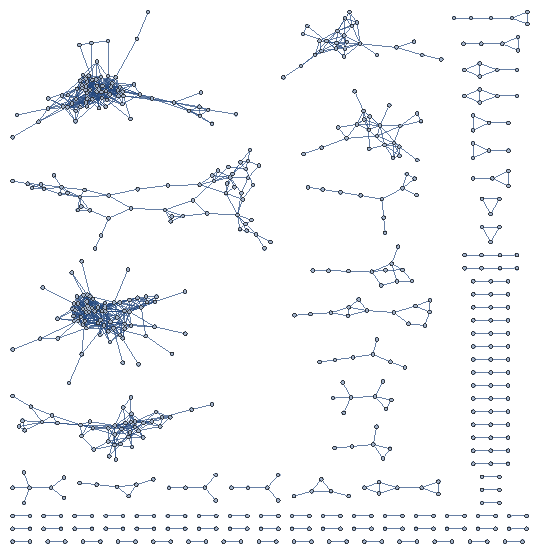
\includegraphics[scale=0.6]{images/atm_graph.pdf}
\caption{\label{fig:graph}Graph representation of the potential conflicts: each node represent a flight
and two nodes have a connection if there is at least one potential conflict. Each graph represent a connected
component of the original NAT dataset.}
\end{figure}
%
\noindent As one can see, large part of the connected components is composed of only few flights.
As shown in \figurename~\ref{fig:cc}, $90\%$ of the connected components has a number of flights which is
smaller than $10$.
%
\begin{figure}[h!]
\centering
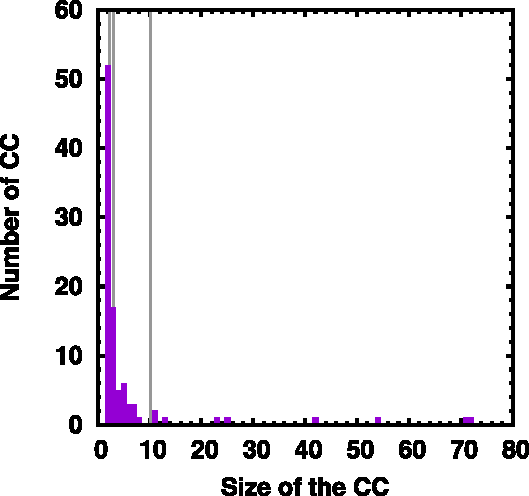
\includegraphics[scale=0.8]{images/cc_hist_mindist030_mintime060.pdf}
\caption{\label{fig:cc}Histogram representing the number of flights in each connected component (cc). The
three horizontal lines represent respectively the $50\%$, the $65\%$ and the $90\%$ of the distribution.}
\end{figure}

\section*{Departure delay-only model on DW2X}

As a first step to understand the power of \DW~quantum annealer in solving the ATM problem, we focused
on a simplified version we called ``departure delay-only'' formulation. In this formulation of the
ATM problem, we still use the NAT dataset of conflicts but the potential conflicts are solved by
changing the departure delay only. This formulation greatly simplifies the QUBO formula so that 
almost $70\%$ of the total flights can be resolved using the \DW~(see \figurename~\ref{fig:solvable_dw2x}).
%
\begin{figure}[h!]
\centering
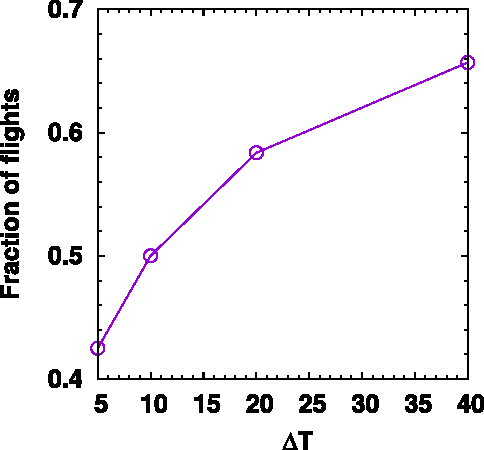
\includegraphics[scale=0.8]{images/fraction-flights-solvable-dw2x.pdf}
\caption{\label{fig:solvable_dw2x}Fraction of flights solvable by using the \DW~quantum annealer. Here
$\Delta T$ is the discretization used for the delays.}
\end{figure}
%
Since \DW~is a quantum heuristic, it can give with a certain probability $p$ the optimal set of initial 
delays. The probability $p$ depends on different free parameters of the \DW~quantum annealer 
that can be simultaneously and independently tuned. At the moment, we are working on optimizing these
free parameters and maximize the likelihood of the \DW~in finding the optimal set of departure delays.
In \figurename~\ref{fig:prob_dw2x} we show the probability of success of the \DW~in finding the 
optimal set of departure delays.
%
\begin{figure*}[h!]
\centering
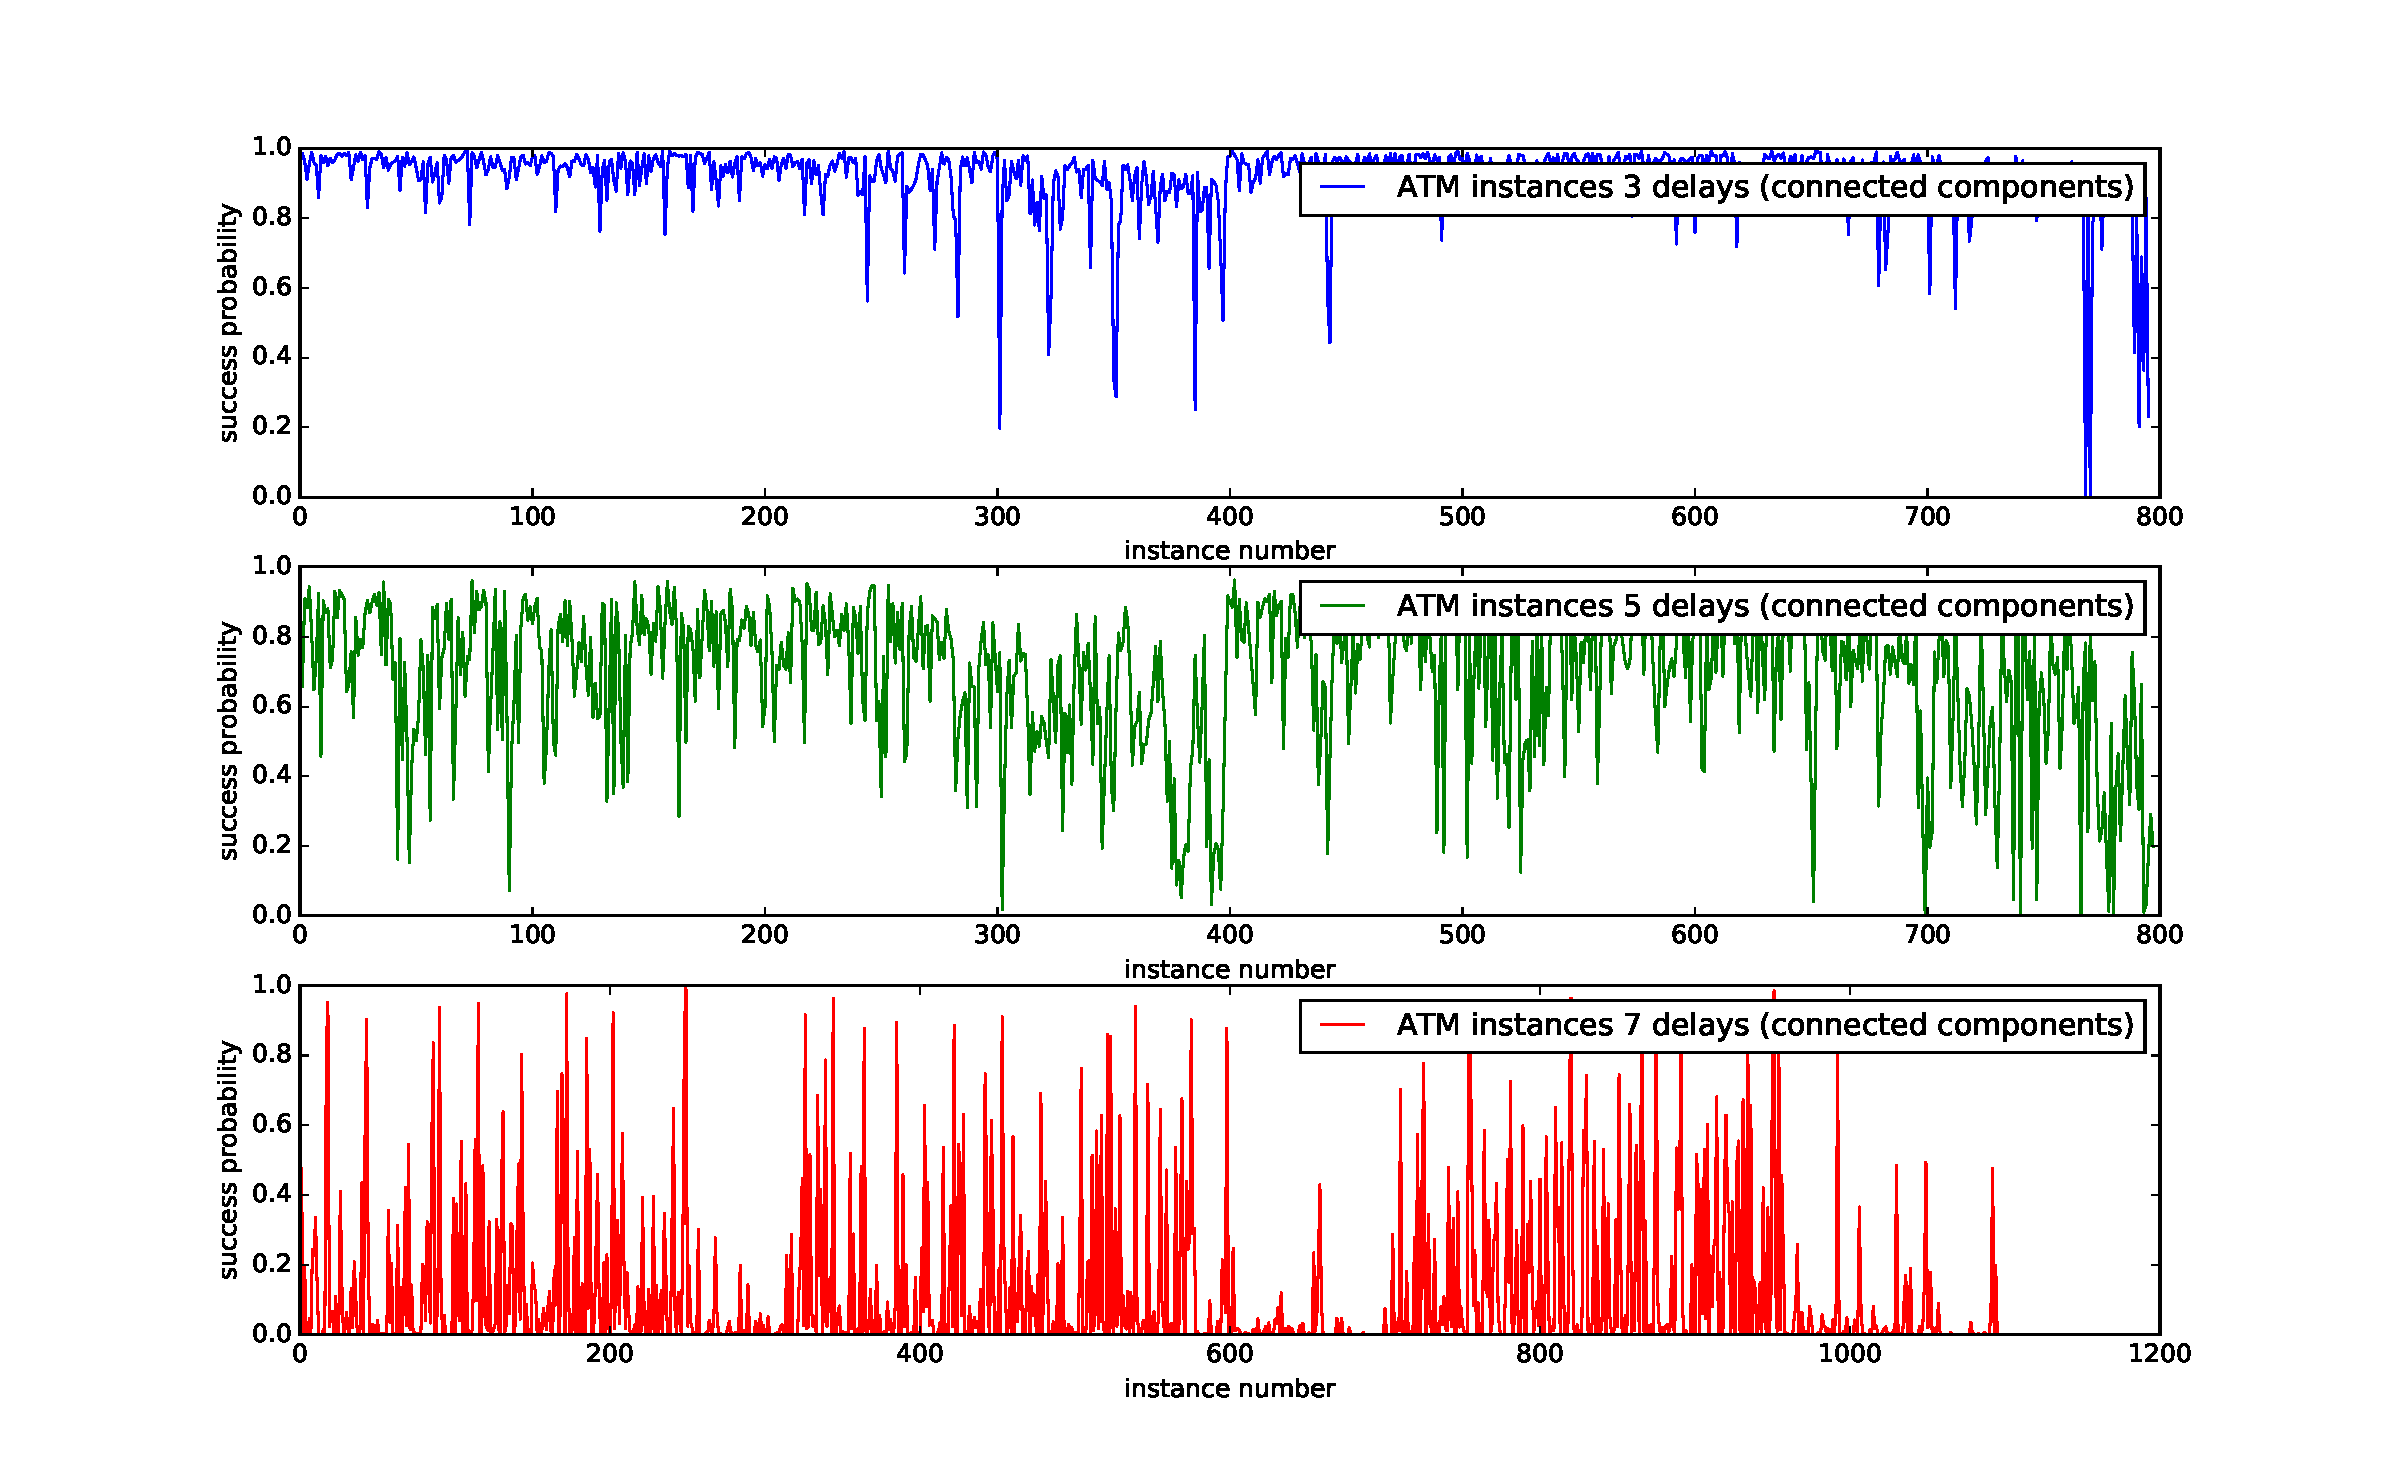
\includegraphics[scale=0.4]{images/prob_dwave.pdf}
\caption{\label{fig:prob_dw2x}Probability of the \DW~quantum annealer in finding the optimal set
of departure delays by varying some free parameters of the model.}
\end{figure*}
%
Given the small sizes we are testing at the moment, we used an exact solver to compare the results from
\DW~quantum annealer.

\section*{Next steps}

Here follows the next steps we are planning to pursue:
\begin{enumerate}
  \item Find optimal parameters for \DW~quantum annealer in order to maximize its probability of success.
  \item Assess if, and in what conditions, the \DW~quantum annealer can be used to solve the ATM problem.
  \item Using classical solvers, we want to compare the solutions of the discrete QUBO model we have devised
        with other continuous solvers like Olga's solver.
\end{enumerate}

\bibliographystyle{unsrt}
\bibliography{refs.bib}

\end{document}
